% -- Implementation ---------------------------------------

\section{Implementation}

The approach described in the previous section wasn't implemented in a day, obviously. This section will cover some difficulties that came along during the lab.

\subsection{The Fix}
Halfway the lab, a fix was introduced. Setting the physical start addres to 0x120 was now done and did not have to be passed on using \mcode{\_\_DATA\_START}. In order to make the $\rho$-VEX read the pixels in the data memory correct a pointer to the first logical address 0 would be enough.

Unfortunately, this caused us problems for weeks. Since we wanted to let the original x264 file unaltered, we copied the folder and created a new application. The folder was called 'lab2', with the \mcode{pixel.c} file called \mcode{microlab2.c}. The \mcode{lab2.c} file containing the extracted kernel was in the rovex-examples folder because of the \mcode{makefile}, that was also residing there. Now, the fix was only applicable to the original x264 folder, so we still had to deal with the stride issue.

When we found out about this fix, we adjusted the original x264 folder. We commented out the source code of \mcode{pixel_satd_8x4} and put our MicroBlaze kernel code instead. To check whether the pixels were sent to $\rho$-VEX data memory correctly, we pre-defined two pixels in \mcode{pixel.c} to be written to \mcode{rvex-dmemory}. This way, we could have certain expectations when doing a \mcode{hexdump} to examine the registers. Our testpixels are shows in figure \ref{fig:test}.

\begin{figure}
	\centering
	\begin{subfigure} [h] {0.5\textwidth}
		\centering
		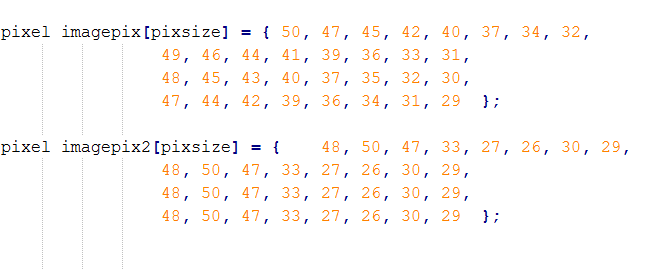
\includegraphics[width=150px]{Pictures/testpixels}
		\caption{Test pixels defined in \mcode{pixel.c}}
		\label{fig:test}
	\end{subfigure}
	\quad
	\begin{subfigure} [h] {0.5\textwidth}
		\centering
		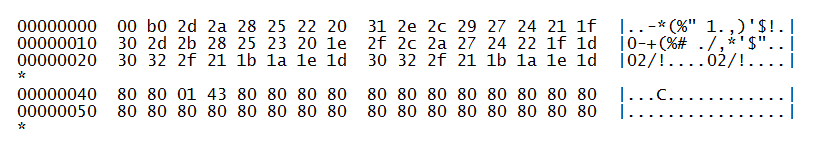
\includegraphics[width=150px]{Pictures/hextest}
		\caption{Hexdump of the testpixels (first two bytes incorrect)}
		\label{fig:testhex}
	\end{subfigure}
	\quad
\caption{Commands for reading from and writing to the $\rho$-VEX}%
\label{}%
\end{figure}


\subsection{Order of Variable Initialization}

After moving our code to the original x264 code and creating test pixels to be used for SATD calculation, a dump of the $\rho$-VEX data memory can been seen in figure \ref{fig:testhex}. As you can see, the first two byte are not matching. At first, we thought this could be because of the fact that another group was running their application at the same FPGA concurrently. However, the value of these bytes remained the same during several runs. 

This unwanted write was caused by the initialization of the \mcode{sum} variable, that has type \mcode{short int} and was stored in the data memory before the pixel. When \mcode{pixel_satd_8x4} tried to find the pixels, it found \mcode{sum} instead of the pixels, causing the program to get stuck in a loop. When changes \mcode{sum} to not being initiazlied, \mcode{datamem} containing the pixels had the first spot at address 120.

\subsection{Endianness}
The MicroBlaze and the $\rho$-VEX understand basic operations like \mcode{open()}, \mcode{close()}, \mcode{read()} and \mcode{write()}. However, they differ in Endiannes. $\rho$-VEX operates in Little Endian, meaning the bytes are read from right to left, as seen in figure \ref{fig:little}. MicroBlaze, on the other hand, operates in Big Endian and thus reads the bytes from left to right (see figure \ref{fig:big}). This becomes an issue when reading the \mcode{result} variable from the data memory, as we will get the bytes in reversed order. This problem is solved by manually reversing the order of the \mcode{result} bytes, realized by the piece of code in figure \ref{fig:swap}.

\begin{figure}
	\centering
	\begin{subfigure} [h] {0.5\textwidth}
		\centering
		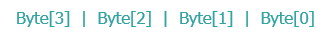
\includegraphics[width=150px]{Pictures/little}
		\caption{Little Endian}
		\label{fig:little}
	\end{subfigure}
	\quad
	\begin{subfigure} [h] {0.5\textwidth}
		\centering
		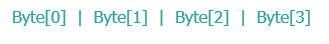
\includegraphics[width=150px]{Pictures/big}
		\caption{Big Endian}
		\label{fig:big}
	\end{subfigure}
	\quad
	\begin{subfigure} [h] {0.5\textwidth}
		\centering
		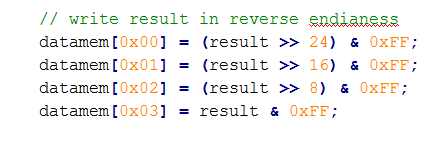
\includegraphics[width=150px]{Pictures/byteswap}
		\caption{Reversing the order of bytes}
		\label{fig:swap}
	\end{subfigure}
\caption{Different reading direction due to Endianness}%
\label{}%
\end{figure}

\subsection{Setting pointer to address 0 using \mcode{lseek}}

When writing pixels to the data memory of the $\rho$-VEX, it is important to know exactly where they end up. This situation can be solved by using \mcode{lseek}, a system call that is used to change the location of the read/write pointer of a file descriptor. When ordering \mcode{lseek(data, 0, SEEK_SET)}, the pointer in the $\rho$-VEX moves to the address that is the start address from his point of view (thus, physical address 0x120). We first made a mistake by putting 0x120 as \mcode{lseek} parameter, which gives an error since the MicroBlaze can not see into the physical address of the $\rho$-VEX. Translating the logical address 0 to the physical address 0x120 is done by the linker and is not of our concern.

